\documentclass{beamer}
\usetheme{Rochester}
\setbeamertemplate{footline}[frame number]

\usepackage[utf8x]{inputenc}
\usepackage[russian]{babel}

\usepackage{tikz-cd}

\usepackage{graphicx}
\graphicspath{{../}}

\iffalse
План:
- История (упор на то, что это язык)
- Основные определения
- Обзор применения в математике
-- В основном, как языка
-- Пара примеров _реального_ применения
-- Примеры duality
-- 
- Связь с теорией типов и логикой, Карри-Говард-Ламбек
- Применение в Хаскеле: монады, free theorems, линзы, линейная логика, ...
- Hask is not a category
- int-cat, HoTT
\fi

\title{Теория категорий}
\author{Никита Лисица}
\date{2020}

\begin{document}

\frame{\titlepage}

\begin{frame}
\frametitle{Немного истории}
\begin{itemize}
\pause
\item Первая половина XX --- развитие алгебраической топологии
\pause
\item 1940е: Эйленберг, Маклейн --- определения категории, функторов, \textit{естественных преобразований}
\pause
\item 1950-60е: Серр, Гротендик, et al. --- бум алгебраической геометрии
\pause
\item 1960е: Маклейн --- моноидальные категории, 2-категории
\pause
\item 1960е: Ловер --- Категорная логика, аксиоматизация категории множеств, топосы
\pause
\item 1960е: Хааг, Кастлер --- Алгебраическая квантовая теория поля
\pause
\item 1970е и далее: \textit{очень много всего}
\end{itemize}
\end{frame}

\begin{frame}
\frametitle{Об обобщениях}
\begin{itemize}
\pause
\item Целое число \pause \begin{math}\Rightarrow\end{math} кольцо целых чисел \begin{math}\mathbb{Z}\end{math} \pause
\item Вещественное число \pause \begin{math}\Rightarrow\end{math} поле вещественных чисел \begin{math}\mathbb{R}\end{math} \pause
\item Непрерывная функция \pause \begin{math}\Rightarrow\end{math} пространство непрерывных функций \begin{math}C(X)\end{math} \pause
\item Конкретные алгебраические структуры \pause \begin{math}\Rightarrow\end{math} универсальная алгебра (изучение структуры с произвольными операциями и аксиомами) \pause
\item Множество* всех колец/полей/пространств/etc \begin{math}\Rightarrow\end{math} \only<8>{???} \pause категория
\end{itemize}
\end{frame}

\begin{frame}
\frametitle{Определение}
\begin{block}{Категория \begin{math}C\end{math} --- это}
\begin{itemize}
\pause
\item Набор \textit{объектов} \begin{math}Ob(C)\end{math}
\pause
\item \begin{math}\forall X,Y \in Ob(C) \end{math} набор \textit{морфизмов}/\textit{стрелок} \begin{math}Hom_C(X,Y)\end{math}
\pause
\item Композиция морфизмов: \begin{math}f\in Hom_C(X,Y), g \in Hom_C(Y,Z) \Rightarrow g\circ f:Hom_C(X,Z)\end{math}
\end{itemize}
\end{block}
\pause
\begin{itemize}
\item Композиция ассоциативна: \begin{math}(h\circ g)\circ f = h\circ (g\circ f)\end{math}
\pause
\item Тождественное отображение: \begin{math}\exists id_X\in Hom_C(X,X)\end{math}
\item \begin{math}id_X \circ f = f \quad g \circ id_X = g\end{math}
\end{itemize}
\end{frame}

\begin{frame}
\frametitle{Определение}
\begin{itemize}
\item Нужно отношение равенства на морфизмах
\item \textit{Не нужно} отношение равенства на объектах
\pause
\item Вместо равенства для объектов используется изоморфизм
\end{itemize}
\end{frame}

\begin{frame}[fragile]
\frametitle{Коммутативные диаграммы}
Композиция:
\begin{equation}
\begin{tikzcd}
X \arrow{r}{f} \onslide*<2->{\arrow[bend right]{rr}[swap]{g\circ f}} & Y \arrow{r}{g} & Z
\end{tikzcd}
\end{equation}
\pause
Диаграмма \textit{коммутативна}, если композиция вдоль любого пути из одной вершины в другую даёт один и тот же морфизм.
\end{frame}

\begin{frame}[fragile]
\frametitle{Коммутативные диаграммы}
Ассоциативность:
\begin{equation}
\begin{tikzcd}
& Y \arrow{r}{g}  \onslide*<2->{\arrow{rrd}}
& Z \arrow{rd}{h}
& \\ X \arrow{ru}{f} \onslide*<2->{\arrow{rru}} \onslide*<3->{\arrow{rrr}{h\circ g\circ f}}
&&& W
\end{tikzcd}
\end{equation}
\end{frame}

\begin{frame}[fragile]
\frametitle{Коммутативные диаграммы}
Тождественное отображение:
\begin{equation}
\begin{tikzcd}
X \arrow{d}[swap]{id_X} \onslide*<2->{\arrow{rd}{f}} & \\
X \arrow{r}{f} & Y
\end{tikzcd}
\end{equation}
\end{frame}

\begin{frame}[fragile]
\frametitle{Изоморфизм}
Морфизмы могут быть обратными друг другу:
\begin{equation}
\begin{tikzcd}
X \arrow{r}{f} \onslide*<2->{\arrow[bend right]{rr}{id_X}} & Y \arrow{r}{g} & X
\end{tikzcd}
\end{equation}
\pause
\begin{equation}f = g^{-1}\end{equation}
\begin{equation}g = f^{-1}\end{equation}
Обратимый морфизм --- изоморфизм
\\
\begin{math}id_X^{-1} = id_X\end{math}
\end{frame}

\begin{frame}
\frametitle{Примеры категорий}
\begin{itemize}
\pause
\item Категория множеств \begin{math}\mathbf{Set}\end{math}
\pause
\item Категория групп \begin{math}\mathbf{Grp}\end{math}
\pause
\item Категория колец \begin{math}\mathbf{Ring}\end{math}
\pause
\item Категория \begin{math}\mathbf{Vect}_K\end{math} векторных пространств над полем \begin{math}K\end{math}
\pause
\item Категория топологических пространств \begin{math}\mathbf{Top}\end{math}
\pause
\item Категория Хаусдорфовых пространств \begin{math}\mathbf{Haus}\end{math}
\pause
\item Категория метрических пространств \begin{math}\mathbf{Met}\end{math}
\pause
\item Категория графов \begin{math}\mathbf{Gph}\end{math}
\pause
\item \textit{Любые математические объекты одной природы}
\end{itemize}
\end{frame}

\begin{frame}
\frametitle{Примеры категорий}
\begin{itemize}
\pause
\item Моноид \begin{math}\Leftrightarrow\end{math} категория с одним объектом
\item Группа \begin{math}\Leftrightarrow\end{math} категория с одним объектом, где все морфизмы обратимы
\item Предпорядок \begin{math}\Leftrightarrow\end{math} категория, где между любыми объектами не более одного морфизма
\item Категория путей графа
\end{itemize}
\end{frame}

\begin{frame}[fragile]
\frametitle{Примеры категорий}
Пустая категория:
\end{frame}

\begin{frame}[fragile]
\frametitle{Примеры категорий}
Категория с одним объектом (и тождественным морфизмом):
\begin{equation}
\begin{tikzcd}
\bullet
\end{tikzcd}
\end{equation}
\end{frame}

\begin{frame}[fragile]
\frametitle{Примеры категорий}
Категория с двумя объектами:
\begin{equation}
\begin{tikzcd}
\bullet & \bullet
\end{tikzcd}
\end{equation}
\end{frame}

\begin{frame}[fragile]
\frametitle{Примеры категорий}
Категория с двумя объектами и морфизмом между ними:
\begin{equation}
\begin{tikzcd}
\bullet \arrow{r} & \bullet
\end{tikzcd}
\end{equation}
\end{frame}

\begin{frame}[fragile]
\frametitle{Примеры категорий}
\begin{equation}
\begin{tikzcd}
\bullet & \bullet \arrow{l} \arrow{r} & \bullet
\end{tikzcd}
\end{equation}
\end{frame}

\begin{frame}
\frametitle{Примеры категорий}
\begin{itemize}
\item Категория высказываний логической системы
\begin{itemize}
\item Морфизмы --- доказательства выводимости
\end{itemize}
\pause
\item Категория типов системы типизации
\begin{itemize}
\item Морфизмы --- термы функций
\end{itemize}
\pause
\item Категория типов языка Haskell --- \begin{math}\mathbf{Hask}\end{math}
\begin{itemize}
\item Морфизмы --- функции
\end{itemize}
\end{itemize}
\end{frame}

\begin{frame}
\frametitle{Приложения}
\begin{itemize}
\item Для большинства приложений --- язык описания явлений и конструкций
\pause
\item Несколько несложных результатов, полезных везде
\pause
\item Алгебраическая геометрия, алгебраическая топология --- невозможны в современном виде без теории категорий
\pause
\item Распространение реального применения на другие области --- активно развивающаяся сфера
\pause
\item Указывает на правильные абстракции \begin{math}\Rightarrow\end{math} помогает проектировать интерфейсы
\end{itemize}
\end{frame}

\begin{frame}[fragile]
\frametitle{Начальный объект категории}
\begin{itemize}
\item \begin{math}\bot \in Ob(C)\end{math} такой, что \begin{math}\forall X \in Ob(C) \quad \exists! f \in Hom_C(\bot, X)\end{math}
\begin{equation}
\begin{tikzcd}
\bot\arrow{r}{\exists!} & \forall X
\end{tikzcd}
\end{equation}
\pause
\item \begin{math}\mathbf{Set}\end{math}: \begin{math}\bot = \varnothing\end{math}
\pause
\item \begin{math}\mathbf{Grp}\end{math}: \begin{math}\bot = 1\end{math}
\pause
\item \begin{math}\mathbf{Vect}_K\end{math}: \begin{math}\bot = \{0\}\end{math}
\pause
\item \begin{math}\mathbf{Hask}\end{math}: \begin{math}\bot = \text{Data.Void}\end{math}
\end{itemize}
\end{frame}

\begin{frame}[fragile]
\frametitle{Терминальный объект категории}
\begin{equation}
\begin{tikzcd}
\forall X \arrow{r}{\exists!} & \top
\end{tikzcd}
\end{equation}
\begin{itemize}
\pause
\item \begin{math}\mathbf{Set}\end{math}: \begin{math}\top = \{\bullet\}\end{math}
\pause
\item \begin{math}\mathbf{Grp}\end{math}: \begin{math}\top = 1\end{math}
\pause
\item \begin{math}\mathbf{Vect}_K\end{math}: \begin{math}\top = \{0\}\end{math}
\pause
\item \begin{math}\mathbf{Hask}\end{math}: \begin{math}\top = ()\end{math}
\pause
\item Получается «переворачиванием стрелок» из определения начального объекта
\end{itemize}
\end{frame}

\begin{frame}[fragile]
\frametitle{Произведение объектов в категории}
\begin{equation}
\begin{tikzcd}
X & \arrow{l} X\times Y \arrow{r} & Y \\
& \forall A \arrow{ul}{\forall} \arrow{ur}[swap]{\forall} \arrow{u}{\exists!}
\end{tikzcd}
\end{equation}
\begin{itemize}
\pause
\item \begin{math}\mathbf{Set}\end{math}: \begin{math}X \times Y\end{math}
\pause
\item \begin{math}\mathbf{Grp}\end{math}: \begin{math}X \times Y\end{math}
\pause
\item \begin{math}\mathbf{Vect}_K\end{math}: \begin{math}X \oplus Y\end{math}
\pause
\item \begin{math}\mathbf{Hask}\end{math}: \begin{math}(X, Y)\end{math}
\end{itemize}
\end{frame}

\begin{frame}[fragile]
\frametitle{Копроизведение (сумма) объектов в категории}
\begin{equation}
\begin{tikzcd}
X \arrow{r} \arrow{dr}[swap]{\forall} & X+Y \arrow{d}{\exists!} & \arrow{l} Y \arrow{dl}{\forall} \\
& \forall A 
\end{tikzcd}
\end{equation}
\begin{itemize}
\pause
\item \begin{math}\mathbf{Set}\end{math}: \begin{math}X \coprod Y\end{math}
\pause
\item \begin{math}\mathbf{Grp}\end{math}: \begin{math}X * Y\end{math}
\pause
\item \begin{math}\mathbf{Vect}_K\end{math}: \begin{math}X \oplus Y\end{math}
\pause
\item \begin{math}\mathbf{Hask}\end{math}: \begin{math}\text{Either X Y}\end{math}
\pause
\item Получается «переворачиванием стрелок» из определения произведения
\end{itemize}
\end{frame}

\begin{frame}[fragile]
\frametitle{Функтор}
\begin{block}{Функтор \begin{math}F: C \rightarrow D\end{math} --- это}
\begin{itemize}
\pause
\item Отображение на объектах: \begin{math}F: Ob(C) \rightarrow Ob(D)\end{math}
\pause
\item Отображение на морфизмах: \begin{math}F: Hom_C(X,Y) \rightarrow Hom_D(F(X),F(Y))\end{math}
\end{itemize}
\end{block}
\pause
Переводит композицию в композицию: \begin{math}F(g\circ f) = F(g) \circ F(f)\end{math}
\pause
\begin{equation}
\begin{tikzcd}
X \arrow{r}{f} \arrow{rd}[swap]{g\circ f} & Y \arrow{d}{g} && F(X) \arrow{r}{F(f)} \arrow{rd}[swap]{F(g\circ f)} & F(Y) \arrow{d}{F(g)} \\
& Z &&& F(Z)
\end{tikzcd}
\end{equation}
\pause
Переводит тождественное в тождественное: \begin{math}F(id_X) = id_{F(X)}\end{math}
\end{frame}

\begin{frame}[fragile]
\frametitle{Функтор: свойства}
Переводит коммутативные диаграммы в коммутативные диаграммы:
\begin{equation}
\begin{tikzcd}
X \arrow{r}{f} \arrow{d}[swap]{i} & Y \arrow{d}{g} && F(X) \arrow{r}{F(f)} \arrow{d}[swap]{F(i)} & F(Y) \arrow{d}{F(g)} \\
W \arrow{d}[swap]{j} & Z \arrow{dl}{h} && F(W) \arrow{d}[swap]{F(j)} & F(Z) \arrow{dl}{F(h)} \\
T &&& F(T)
\end{tikzcd}
\end{equation}
\pause
\begin{equation}
h\circ g\circ f=j\circ i \quad \Longrightarrow \quad F(h)\circ F(g)\circ F(f) = F(j)\circ F(i)
\end{equation}
\end{frame}

\begin{frame}[fragile]
\frametitle{Функтор: свойства}
Переводит изоморфизм в изоморфизм:
\begin{equation}
\begin{tikzcd}
X \arrow{r}{f} \arrow{rd}[swap]{id_X} & Y \arrow{d}{g} && F(X) \arrow{r}{F(f)} \arrow{rd}[swap]{id_{F(X)}} & F(Y) \arrow{d}{F(g)} \\
& X &&& F(X)
\end{tikzcd}
\end{equation}
\pause
\begin{equation}
F(g) = F(f^{-1}) = F(f)^{-1} = F(g)
\end{equation}
\end{frame}

\begin{frame}
\frametitle{Функтор: примеры}
\begin{itemize}
\pause
\item Тождественный функтор \begin{math}Id_C\end{math}
\pause
\item Постоянный функтор
\pause
\item Множество подмножеств \begin{math}X \mapsto 2^X\end{math}
\pause
\item Свободный моноид/группа/etc, свободные функторы
\pause
\item Забывающие функторы, например \begin{math}\mathbf{Grp} \rightarrow \mathbf{Set}\end{math}
\pause
\item Если категории --- частичные порядки, то функтор --- монотонная функция
\pause
\item Если категории --- моноиды/группы, то функтор --- гомоморфизм моноидов/групп
\pause
\item Функторы в Хаскеле: \begin{math}\mathbf{Hask} \rightarrow \mathbf{Hask}\end{math}
\begin{itemize}
\item Отображение на морфизмах --- \texttt{fmap}
\end{itemize}
\end{itemize}
\end{frame}

\begin{frame}
\frametitle{Изоморфизм категорий}
Изоморфизм категорий --- обратимый функтор:
\begin{equation}F : C \rightarrow D\end{equation}
\begin{equation}G : D \rightarrow C\end{equation}
\begin{equation}\forall X \in Ob(C) \quad G(F(X)) = X\end{equation}
\begin{equation}\forall f:X\rightarrow Y \quad G(F(f)) = f\end{equation}
\pause
Используется равенство объектов --- плохое определение!
\pause
Лучше рассматривать \textit{эквивалентность} категорий. \\
Для этого нужны \textit{естественные преобразования}.
\end{frame}

\begin{frame}[fragile]
\frametitle{Естественные преобразования}
\begin{itemize}
\item Функторы --- между категориями
\pause
\item Естественные преобразования --- между функторами
\end{itemize}
\pause
\begin{equation}F, G: C \rightarrow D\end{equation}
\pause
\begin{equation}\eta: F \Rightarrow G\end{equation}
\begin{equation}\eta_X:F(X) \rightarrow G(X) \quad (X\in Ob(C))\end{equation}
\pause
\begin{equation}
\begin{tikzcd}
X \arrow{d}{f} && F(X) \arrow{d}[swap]{F(f)} \arrow{r}{\eta_X} & G(X) \arrow{d}{G(f)} \\
Y && F(Y) \arrow{r}{eta_Y} & G(Y)
\end{tikzcd}
\end{equation}
\begin{equation}\eta_Y \circ F(f) = G(f) \circ \eta_X\end{equation}
\end{frame}

\begin{frame}[fragile]
\frametitle{Естественные преобразования: пример}
Определитель матрицы: \begin{math}\det:M(n,R) \rightarrow R\end{math}
\pause
\begin{equation}
\begin{tikzcd}
M(n,R) \arrow{r}{f} \arrow{d}[swap]{\det} & M(n,S) \arrow{d}{\det} \\
R \arrow{r}{f} & S
\end{tikzcd}
\end{equation}
\pause
В частности:
\begin{itemize}
\item \begin{math}\det(\overline A) = \overline{\det(A)}\end{math}
\item \begin{math}\det(A \operatorname{mod} p) = \det(A) \operatorname{mod} p\end{math}
\end{itemize}
\pause
Мораль: естественные преобразования --- то, что определяется общей формулой, вне зависимости от параметров
\newline
\pause
Естественные преобразования в Хаскеле --- параметрически полиморфные функции \texttt{f: F a -> G a}
\end{frame}

\begin{frame}
\frametitle{Естественный изоморфизм}
\begin{math}\eta\end{math} --- естественный изоморфизм, если все \begin{math}\eta_X\end{math} --- изоморфизмы.
\end{frame}

\begin{frame}
\frametitle{Эквивалентность категорий}
\textit{C} и \textit{D} эквивалентны, если существуют функторы \begin{math}F:C\rightarrow D\end{math} и \begin{math}G:D\rightarrow C\end{math} такие, что 
\begin{itemize}
\item \begin{math}G\circ F\end{math} естественно изоморфно \begin{math}Id_C\end{math}
\item \begin{math}F\circ G\end{math} естественно изоморфно \begin{math}Id_D\end{math}
\end{itemize}
\pause
\begin{itemize}
\item Может быть разное количество изоморфных объектов, но суть остаётся
\item \textit{Скелет} категории --- выбираем по одному объекту из набора изоморфных
\item Любая категория эквивалентна скелету
\end{itemize}
\end{frame}

\begin{frame}[fragile]
\frametitle{Двойственная (opposite) категория}
\begin{itemize}
\item \begin{math}Ob(C^{op}) = Ob(C)\end{math}
\item \begin{math}Hom_{C^{op}}(X, Y) = Hom_C(Y,X)\end{math}
\pause
\begin{equation}
\begin{tikzcd}
C: && X \arrow{r}{f} & Y \\
C^{op}: && X & \arrow{l}[swap]{f} Y
\end{tikzcd}
\end{equation}
\pause
\item Суть --- та же, стрелки --- перевёрнуты
\item Превращает все понятия в двойственные
\end{itemize}
\end{frame}

\begin{frame}
\frametitle{Двойственная категория: примеры}
\begin{itemize}
\item Категория коммутативных колец \begin{math}\leftrightarrow\end{math} категория аффинных схем
\pause
\item (Представление Гельфанда) Категория коммутативных \begin{math}C^*\end{math}-алгебр \begin{math}\leftrightarrow\end{math} категория компактных хаусдорфовых пространств
\pause
\begin{itemize}
\item \begin{math}\Rightarrow\end{math} Некоммутативная геометрия
\end{itemize}
\pause
\item (Теорема Стоуна) Категория булевых алгебр \begin{math}\leftrightarrow\end{math} категория пространств Стоуна
\pause
\item (Двойственность Понтрягина) Категория локально компактных абелевых групп двойственна самой себе
\pause
\begin{itemize}
\item Обобщение рядов Фурье, дискретных и непрерывных преобразований Фурье
\end{itemize}
\end{itemize}
\end{frame}

\begin{frame}
\frametitle{Free theorems}
\begin{itemize}
\item Параметрически полиморфные функции --- естественные преобразования функторов
\item Можно делать вывод о свойствах функции, зная её тип
\end{itemize}
\pause
\begin{itemize}
\item \texttt{f :: a -> a}
\begin{itemize}
\item \texttt{f x = x}
\end{itemize}
\pause
\item \texttt{f :: a -> (a,a)}
\begin{itemize}
\item \texttt{f x = (x,x)}
\end{itemize}
\pause
\item \texttt{f :: (a,b) -> (b,a)}
\begin{itemize}
\item \texttt{f (x,y) = (y,x)}
\end{itemize}
\pause
\item \texttt{f :: a -> [a]}
\begin{itemize}
\item \texttt{f = replicate n}
\end{itemize}
\pause
\item \texttt{f :: [a] -> Int}
\begin{itemize}
\item \texttt{f = g . length}
\end{itemize}
\end{itemize}
\end{frame}

\begin{frame}
\frametitle{Моноидальные категории}
Задано \textit{произведение} объектов: функтор \begin{math}\otimes:C\times C\rightarrow C\end{math} и нейтральный объект \begin{math}I\otimes X \cong X \otimes I \cong X\end{math}
\begin{itemize}
\item \begin{math}\mathbf{Set}, \otimes = \times, I = \{\bullet\}\end{math}
\item \begin{math}\mathbf{Set}, \otimes = \coprod, I = \varnothing\end{math}
\item \begin{math}\mathbf{Vect}_K, \otimes = \otimes, I = K\end{math}
\item Категория функторов из категории в саму себя (\textit{эндофункторов}) \begin{math}\mathbf{End}(C), \otimes = \circ, I = Id_C\end{math}
\end{itemize}
\end{frame}

\begin{frame}
\frametitle{Моноид в моноидальной категории}
Больше структуры --- новые определения!
\begin{block}{Моноид \textit{M} --- это}
\begin{itemize}
\item Умножение: \begin{math}\mu: M\otimes M\rightarrow M\end{math}
\item Единица: \begin{math}\eta: I \rightarrow M\end{math}
\end{itemize}
\end{block}
Аксиомы (ассоциативность, нейтральный элемент) выражаются как диаграммы
\newline
Моноиды в \begin{math}\mathbf{Set}, \times, \{\bullet\}\end{math} --- обычные моноиды из алгебры
\end{frame}

\begin{frame}
\frametitle{Монады}
Монады --- моноиды в категории эндофункторов.
\begin{itemize}
\item \begin{math}\mu:M(M(X)) \rightarrow M(X)\end{math}
\begin{itemize}
\item \texttt{join :: Monad m => m (m a) -> m a}
\end{itemize}
\item \begin{math}\eta:X \rightarrow M(X)\end{math}
\begin{itemize}
\item \texttt{return :: Monad m => a -> m a}
\end{itemize}
\end{itemize}
\end{frame}

\begin{frame}
\frametitle{Тройки Клейсли}
\begin{itemize}
\item Эквивалентны монадам
\item Вместо \begin{math}\mu\end{math} операция \begin{math}f: X \rightarrow M(Y) \quad \Longrightarrow \quad f^*:M(X) \rightarrow M(Y)\end{math}
\item \texttt{flip (>{}>=) :: Monad m => (a -> m b) -> (m a -> m b)}
\end{itemize}
\end{frame}

\begin{frame}
\frametitle{Струнные диаграммы}
\begin{itemize}
\item Пенроуз, Фейнман, ...
\item Объекты --- струны/нити, морфизмы --- блоки
\end{itemize}
\begin{figure}
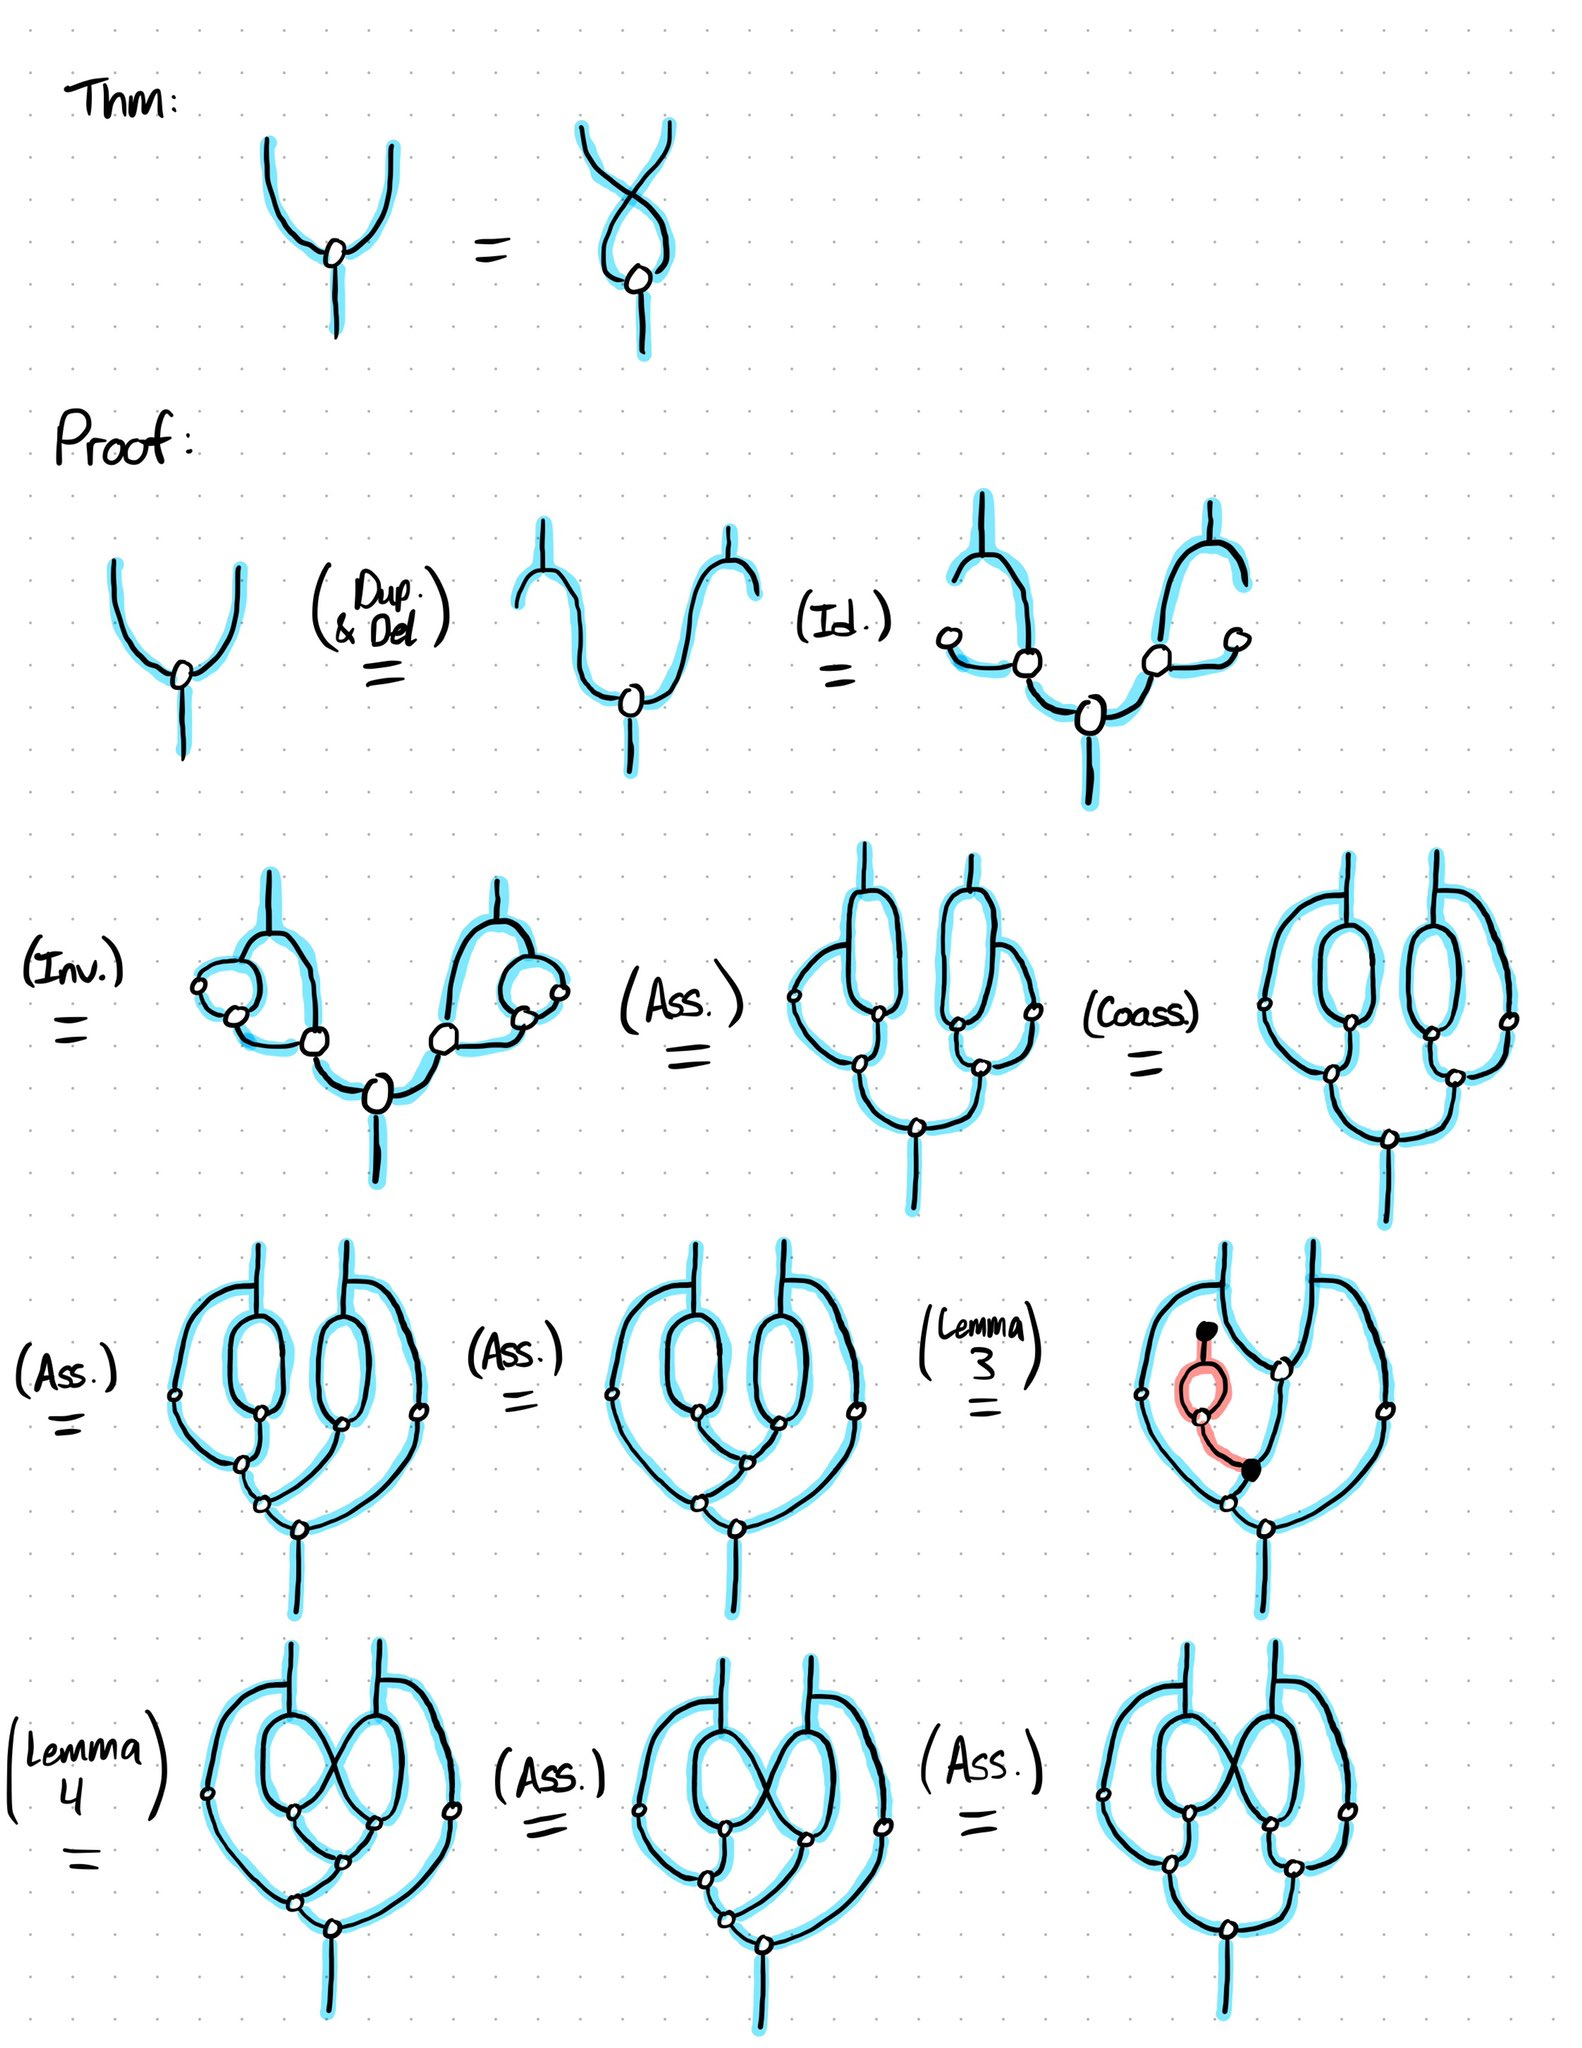
\includegraphics[height=5cm]{addition-commutative-1.jpeg}
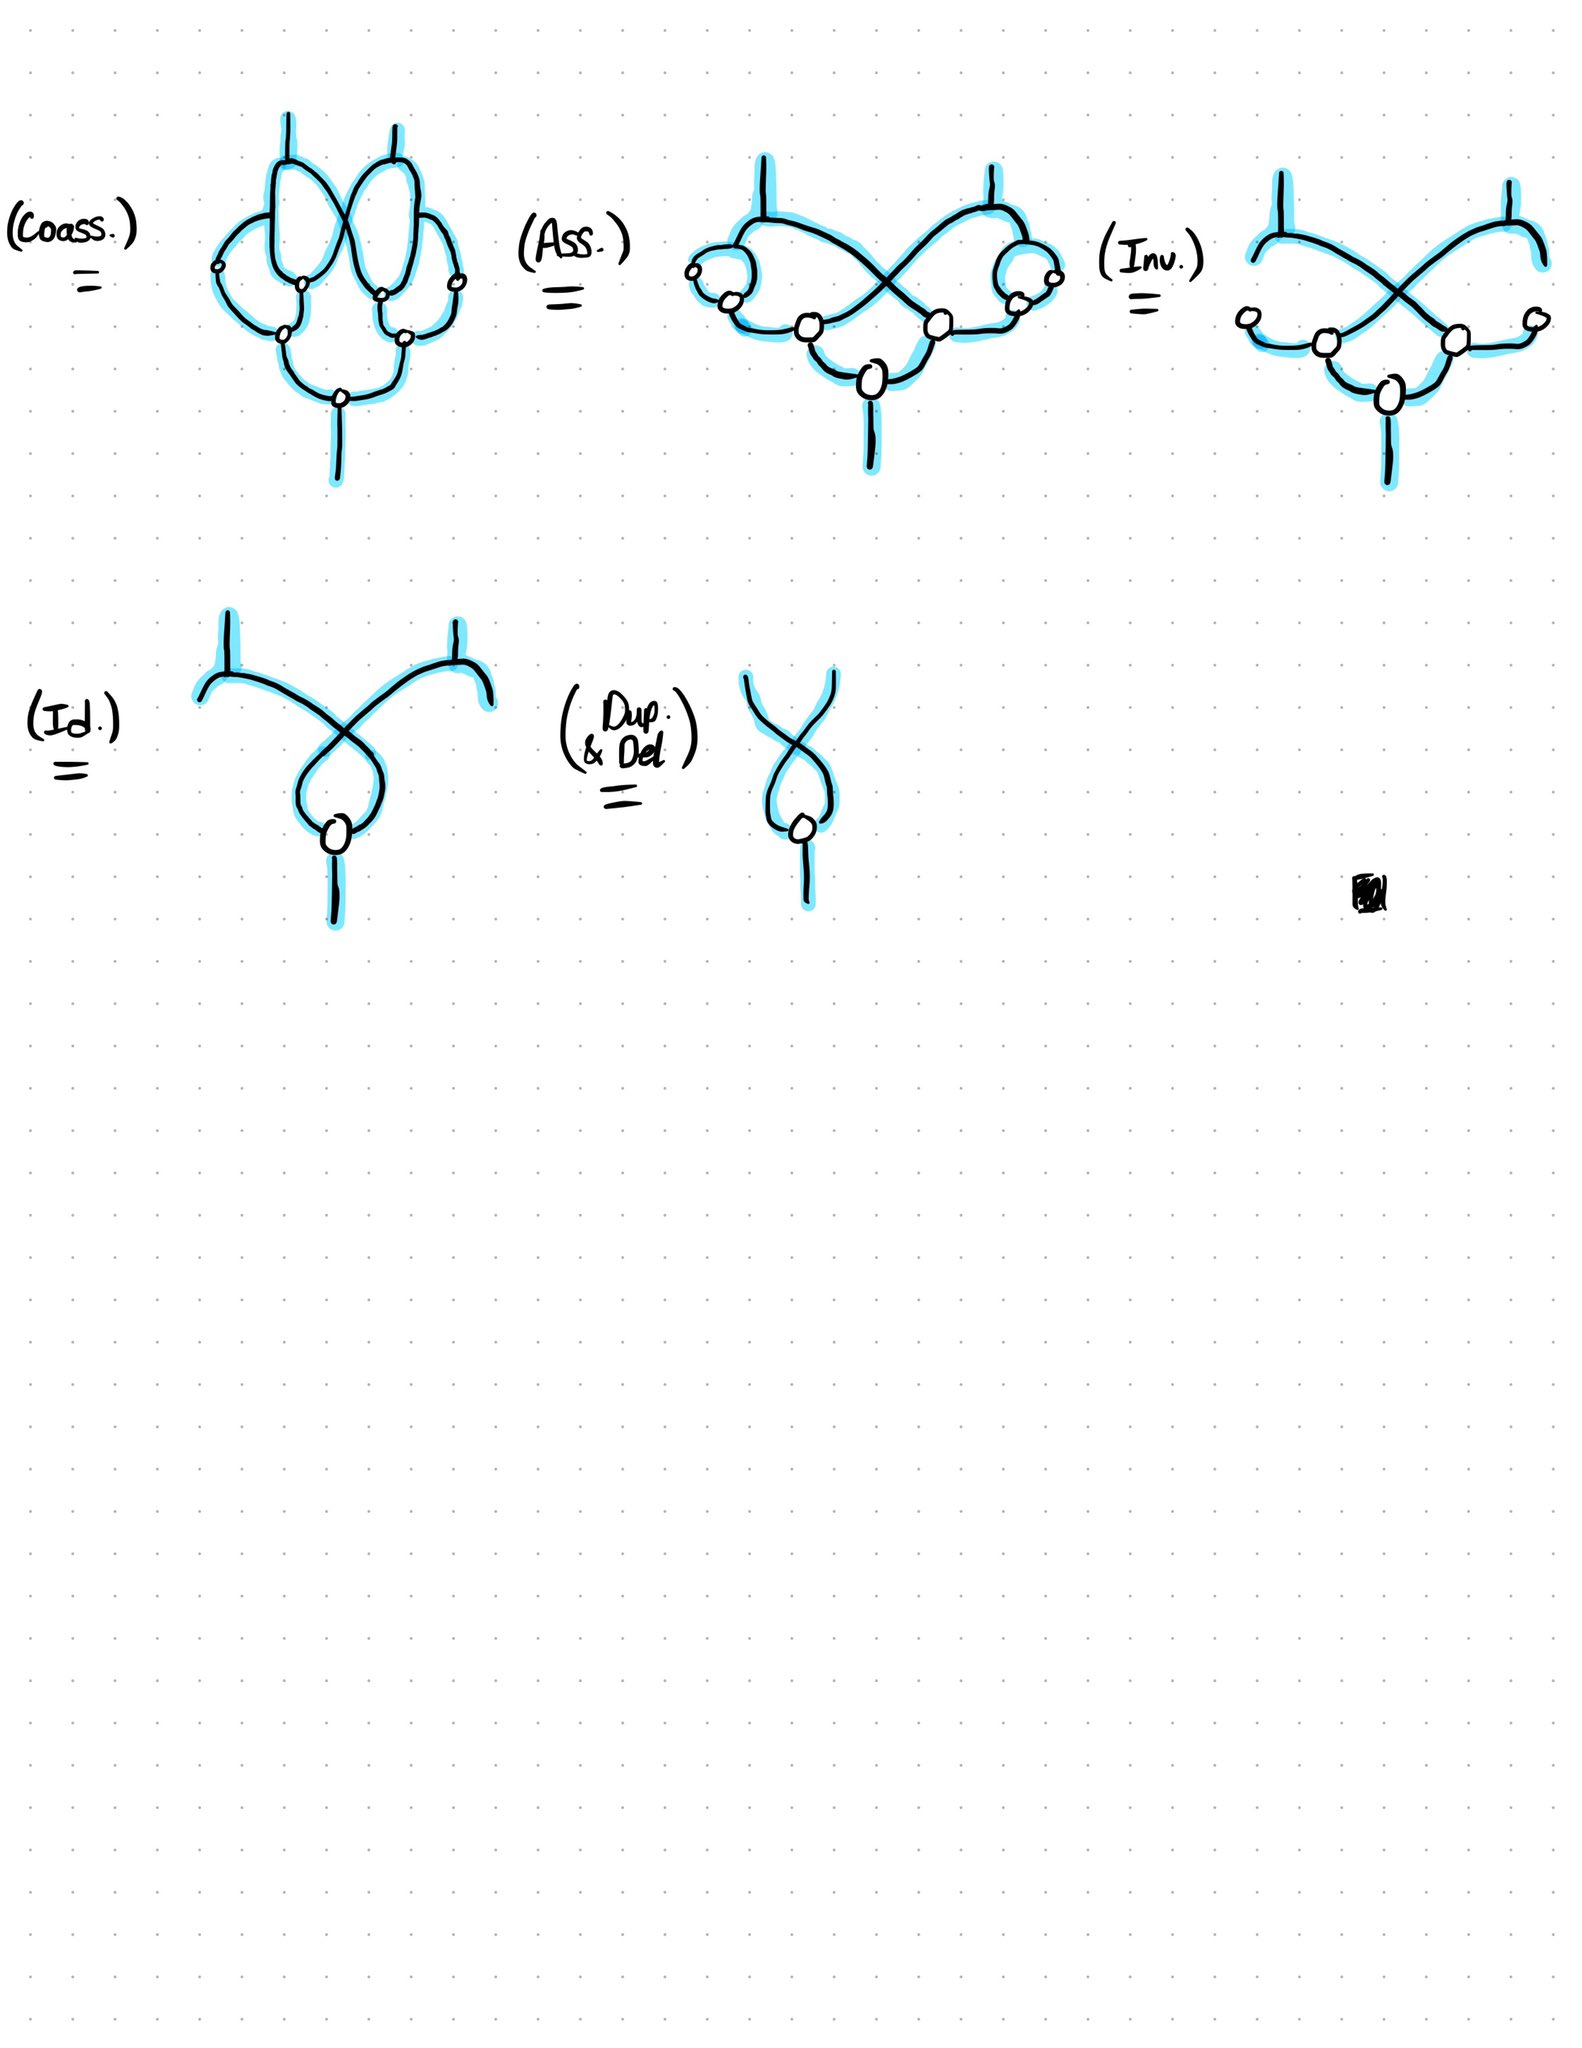
\includegraphics[height=5cm]{addition-commutative-2.jpeg}
\end{figure}
Jordan Sawdy, \texttt{twitter.com/pseudofunctor}
\end{frame}

\begin{frame}
\frametitle{Соответствие Карри-Говарда}
\begin{tabular}{|p{3cm}|p{3cm}|}
\hline
Интуиционистская логика & Просто типизированное лямбда-исчисление \\
\hline
Линейная логика & Линейные типы \\
\hline
Интуиционистская логика первого порядка & Зависимые типы \\
\hline
\end{tabular}
\end{frame}

\begin{frame}
\frametitle{Соответствие Карри-Говарда-Ламбека}
\begin{tabular}{|p{3cm}|p{3cm}|p{3cm}|}
\hline
Интуиционистская логика & Просто типизированное лямбда-исчисление & Декартово-замкнутые  категории \\
\hline
Линейная логика & Линейные типы & Моноидальные категории \\
\hline
Интуиционистская логика первого порядка & Зависимые типы & Локально декартово-замкнутые категории \\
\hline
\end{tabular}
\newline
\newline
nLab: computational trinitarianism
\end{frame}

\begin{frame}
\frametitle{Hask is not a category}
\begin{itemize}
\item Для определения категории нужно уметь сравнивать морфизмы
\item Что означает равенство функций в Хаскеле?
\pause
\begin{itemize}
\item Синтаксически равные термы \pause --- \texttt{fst != swap . snd}
\pause
\item Денотационно равные функции \pause --- никто не описал денотационную семантику Хаскеля
\end{itemize}
\pause
\item Можно ли жить \textit{без} равенства морфизмов? \pause Да, если заменить равенство на \textit{изоморфизм}.
\end{itemize}
\end{frame}

\begin{frame}
\frametitle{(слабые) 2-категории}
\begin{itemize}
\item Объекты
\item Морфизмы между объектами
\pause
\item 2-морфизмы между обычными морфизмами
\pause
\item Аксиомы для морфизмов (ассоциативность, тождественный морфизм) выполняются \textit{с точностью до 2-изоморфизма}
\pause
\item Похоже на триангуляцию: объекты --- точки, морфизмы --- рёбра, 2-морфизмы --- грани
\begin{itemize}
\item Связь с алгебраической топологией
\end{itemize}
\pause
\item Нужно уметь сравнивать 2-морфизмы!
\end{itemize}
\end{frame}

\begin{frame}
\frametitle{\begin{math}\infty\end{math}-категории}
\begin{itemize}
\item Объекты
\item 1-морфизмы между объектами, аксиомы с точностью до 2-изоморфизма
\item 2-морфизмы между 1-морфизмами, аксиомы с точностью до 3-изоморфизма
\item 3-морфизмы между 2-морфизмами, ...
\item ...
\pause
\item С каждым шагом аксиомы (coherence diagrams) всё сложнее --- область активных исследований
\item Модель для гомотопической теории типов
\end{itemize}
\end{frame}

\begin{frame}
\frametitle{Ссылки}
\begin{itemize}
\item nLab: \texttt{ncatlab.org}
\item Saunders Mac Lane, \textit{Categories for the Working Mathematician}
\item Bartosz Milewski, \textit{Category Theory for Programmers}
\item John C. Baez, Mike Stay, \textit{Physics, Topology, Logic and Computation: A Rosetta Stone}
\item Peter Selinger, \textit{A survey of graphical languages for monoidal categories}
\end{itemize}
\end{frame}

\end{document}
